\documentclass[tikz,border=10pt]{standalone}
% Shared style for all Speed Demon diagrams: one palette, rounded white boxes,
% dark ink, white page (readable on GitHub light and dark).
\hyphenpenalty=10000 \exhyphenpenalty=10000 \tolerance=9999
\usepackage[T1]{fontenc}
\usepackage[scaled=0.95]{helvet}
\renewcommand{\familydefault}{\sfdefault}
\usepackage{tikz}
\usepackage{pgfplots}
\pgfplotsset{compat=1.16}
\usetikzlibrary{arrows.meta,positioning,shapes.geometric,fit,backgrounds,calc}

\definecolor{ink}{HTML}{1F2937}
\definecolor{mute}{HTML}{6B7280}
\definecolor{rule}{HTML}{9CA3AF}
\definecolor{cA}{HTML}{2563EB}   % Track A  blue
\definecolor{cB}{HTML}{D97706}   % Track B  amber
\definecolor{cC}{HTML}{059669}   % Track C  green
\definecolor{cD}{HTML}{7C3AED}   % Track D  violet
\definecolor{warn}{HTML}{DC2626} % fallback / redo path
\definecolor{wash}{HTML}{F3F4F6}

\tikzset{
  every node/.style={font=\small, text=ink},
  >={Stealth[length=2.4mm,width=1.8mm]},
  box/.style={draw=ink, fill=white, rounded corners=3pt, line width=0.7pt,
    align=center, inner sep=5pt, minimum height=12mm, text width=#1},
  box/.default=44mm,
  accent/.style={draw=#1, line width=1.2pt},
  accent/.default=cA,
  hl/.style={fill=#1!10, draw=#1, line width=1.1pt},
  dec/.style={diamond, aspect=2.6, draw=ink, fill=white, line width=0.7pt,
    align=center, inner sep=2pt, text width=#1},
  dec/.default=34mm,
  arr/.style={->, line width=0.9pt, color=ink},
  redo/.style={->, line width=0.9pt, color=warn, dash pattern=on 4pt off 3pt},
  lab/.style={font=\footnotesize, text=mute, inner sep=2pt},
  grp/.style={draw=#1, dashed, line width=0.9pt, rounded corners=6pt, inner sep=9pt,
    fill=#1!4},
  grp/.default=mute,
  grplabel/.style={font=\footnotesize\bfseries, text=#1, inner sep=2pt},
  show background rectangle,
  background rectangle/.style={fill=white, rounded corners=0pt},
}
\pgfplotsset{
  every axis/.append style={font=\small, tick label style={font=\footnotesize},
    axis line style={ink}, tick style={ink}, grid style={rule!50},
    label style={font=\small}, title style={font=\small\bfseries}},
}

% node text: \nt{title}{detail}
\newcommand{\nt}[2]{\textbf{#1}\par\vspace{1pt}{\footnotesize #2}}

\begin{document}
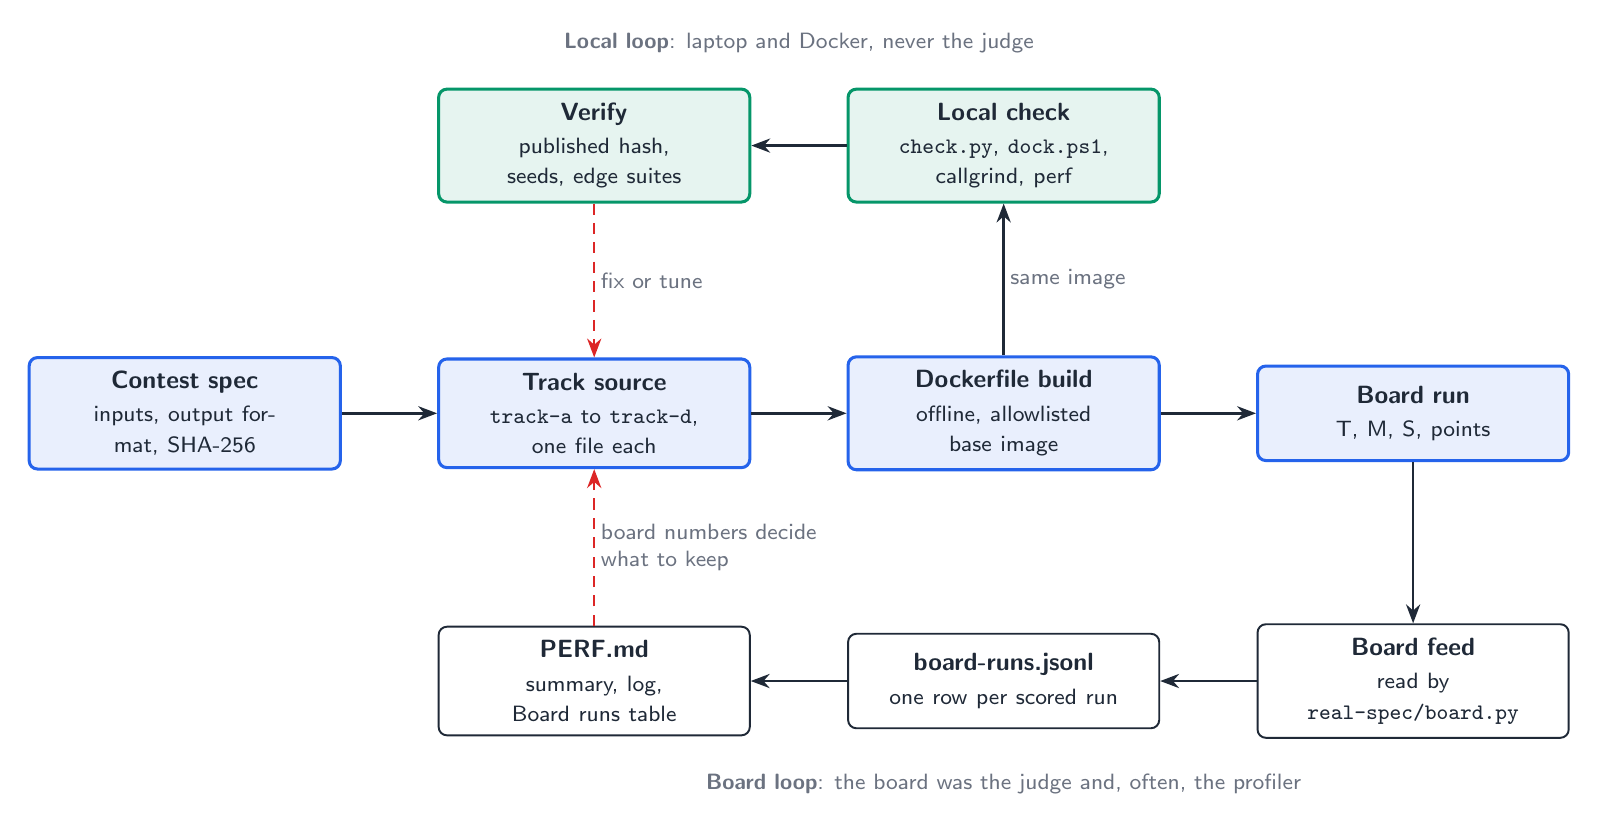
\begin{tikzpicture}
  % main pipeline (row 1) and its return path (row 2)
  \node[box=36mm, hl=cA] (spec) at (0,0)  {\nt{Contest spec}{inputs, output format, SHA-256}};
  \node[box=36mm, hl=cA] (src)  at (5.2,0) {\nt{Track source}{\texttt{track-a} to \texttt{track-d}, one file each}};
  \node[box=36mm, hl=cA] (dock) at (10.4,0) {\nt{Dockerfile build}{offline, allowlisted base image}};
  \node[box=36mm, hl=cA] (run)  at (15.6,0) {\nt{Board run}{T, M, S, points}};

  \node[box=36mm] (feed)  at (15.6,-3.4) {\nt{Board feed}{read by \texttt{real-spec/board.py}}};
  \node[box=36mm] (jsonl) at (10.4,-3.4) {\nt{board-runs.jsonl}{one row per scored run}};
  \node[box=36mm] (perf)  at (5.2,-3.4)  {\nt{PERF.md}{summary, log, Board runs table}};

  % local verification loop (row 0)
  \node[box=36mm, hl=cC] (local) at (10.4,3.4) {\nt{Local check}{\texttt{check.py}, \texttt{dock.ps1}, callgrind, perf}};
  \node[box=36mm, hl=cC] (ver)   at (5.2,3.4)  {\nt{Verify}{published hash, seeds, edge suites}};

  \draw[arr] (spec) -- (src);
  \draw[arr] (src) -- (dock);
  \draw[arr] (dock) -- (run);
  \draw[arr] (run) -- (feed);
  \draw[arr] (feed) -- (jsonl);
  \draw[arr] (jsonl) -- (perf);
  \draw[arr] (dock) -- node[lab, right] {same image} (local);
  \draw[arr] (local) -- (ver);
  \draw[redo] (ver) -- node[lab, right] {fix or tune} (src);
  \draw[redo] (perf) -- node[lab, right, align=left, text width=30mm] {board numbers decide what to keep} (src);
  \node[lab, anchor=south] at (7.8,4.5) {\textbf{Local loop}: laptop and Docker, never the judge};
  \node[lab, anchor=north] at (10.4,-4.5) {\textbf{Board loop}: the board was the judge and, often, the profiler};
\end{tikzpicture}
\end{document}
